\documentclass[12pt,a4paper]{article}
\usepackage{graphics}
\usepackage{csvsimple}
\usepackage[russian,english]{babel}
\usepackage[utf8]{inputenc}
\usepackage[T2A]{fontenc} 
\hoffset -1.6cm 
\textwidth  16.5cm 
\textheight 24cm 
%\topmargin -1cm 
\parskip 8pt plus 1pt minus 1pt 
\setlength{\unitlength}{1cm}
\sloppy
\addto\captionsenglish{
\renewcommand{\contentsname}{{\bf CO}ntents}
\renewcommand{\refname}{Bibliography}
\renewcommand{\figurename}{Figure}
\renewcommand{\tablename}{Table}
\renewcommand{\abstractname}{Abstract}
\renewcommand{\partname}{Section}
\renewcommand{\bottomfraction}{0.5}
\renewcommand{\floatpagefraction}{0.4}
\renewcommand{\textfloatsep}{0.5cm}
\renewcommand{\intextsep}{0.6cm}
\renewcommand{\floatsep}{0.3cm}
}

\begin{document}
%..................................................................
\begin{titlepage}
\par 
\vspace*{-2cm}
\begin{center}
{\sf \Large
\vspace*{1.5cm}
{\Huge Семенов, 8-й семестр, 2017}\\
{ Все, что вы хотели {\small(или не хотели, но сдавать надо)} знать о философии,\\ но боялись спросить}}\\
\vspace*{2cm}
\scalebox{1.2}{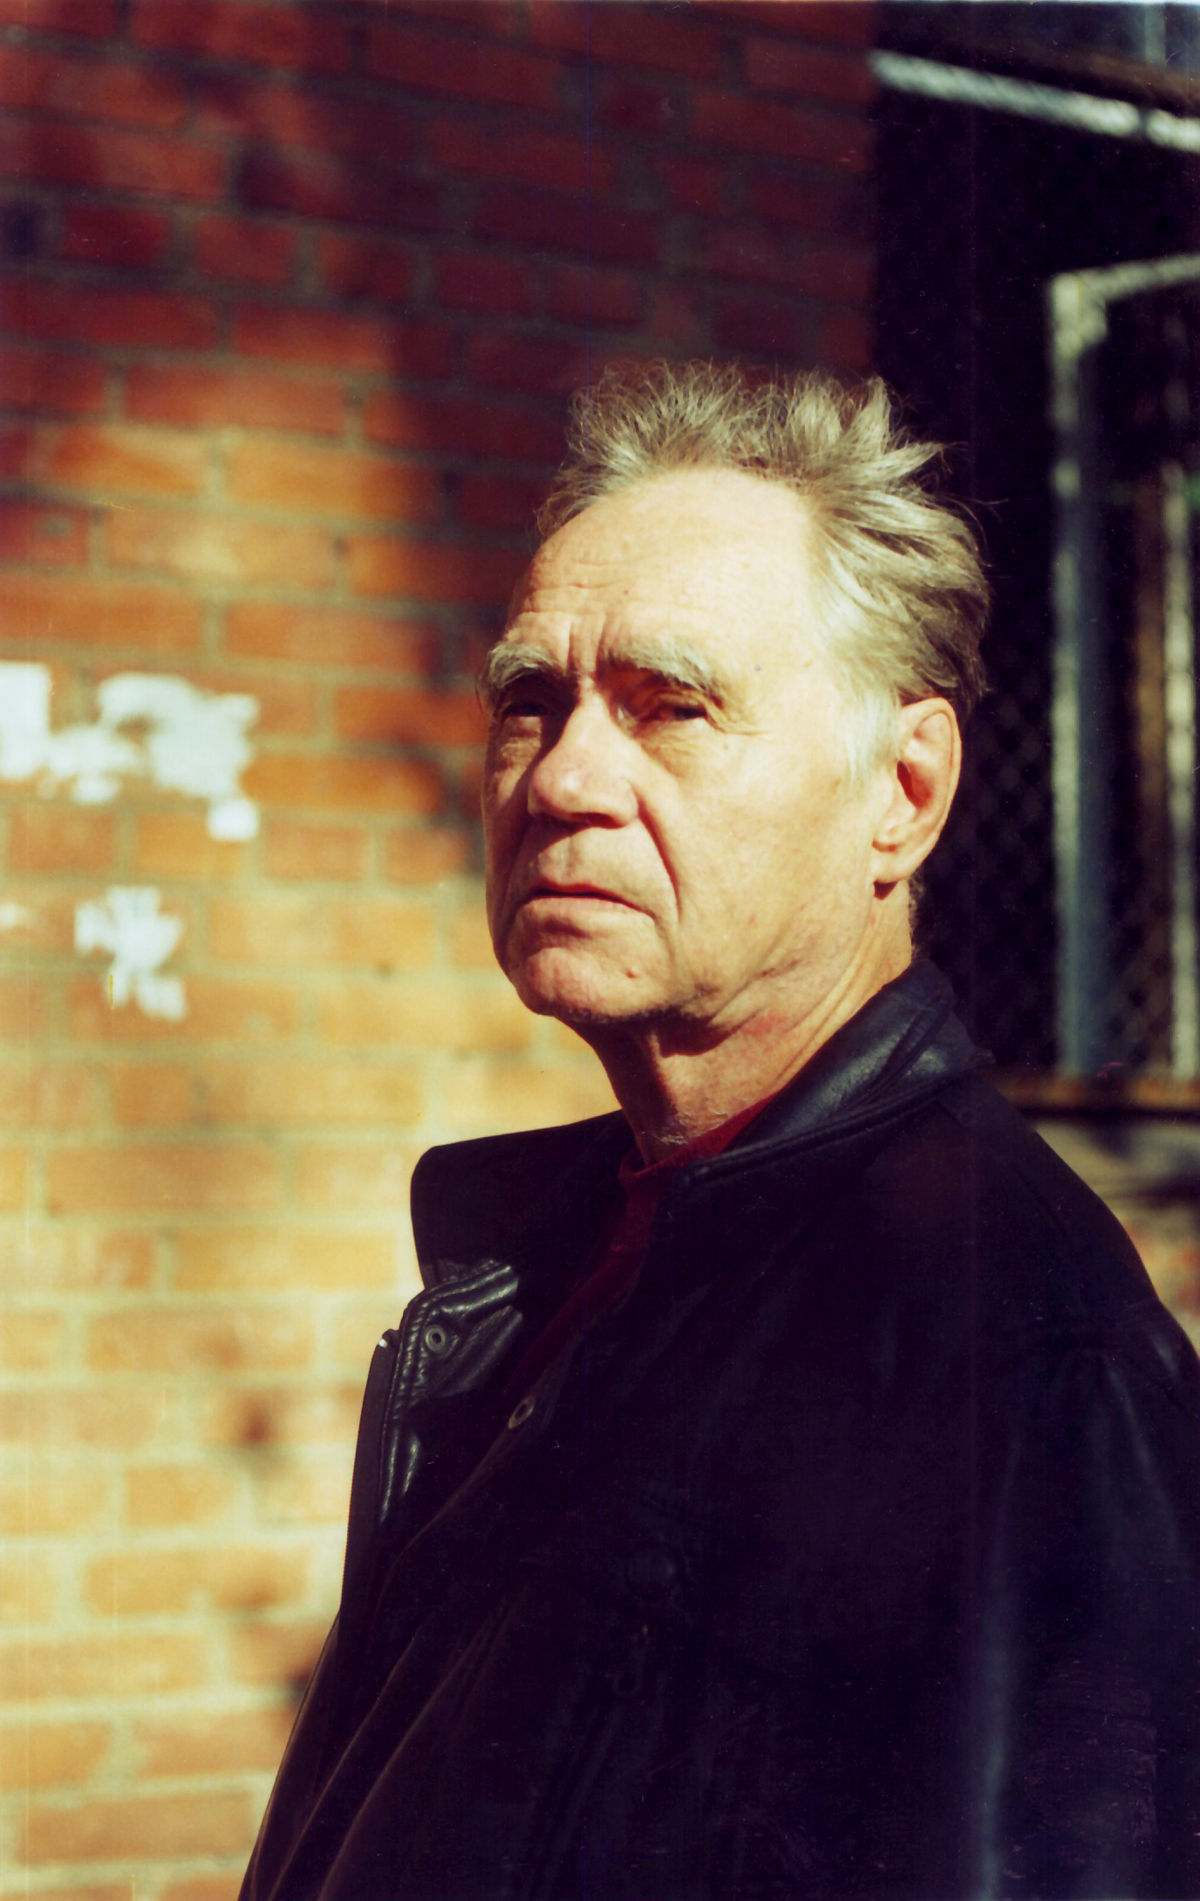
\includegraphics{thegod.png}} 
\begin{flushright}
\sl\small
by Nyaxx11k aka KingKO,\\
Institute for Porn and Pederasts,\\
Chair of Roosterology
\end{flushright}
\end{center}
\end{titlepage}
%..................................................................
\topmargin -1cm 
\hoffset -0.7in 
\textwidth 6.0in 
\textheight 9.0in 
\normalsize 
\pagenumbering{arabic}
%----------------
\tableofcontents
\pagebreak
%----------------

\section{Истина как цель научного исследования. Истина и заблуждение.}
Согласно т.н. "Классическому определению истины", \textbf{истина} - это то, что согласуется с действительностью. 
Соответственно \textbf{заблуждение} - то, что с действительностью не согласуется. \textit{Не ложь - это отрицание истины исключительно в матлогике. В остальных науках это - умышленное введение в заблуждение.}
Ясно, что все науки занимаются поиском истины.
Каждая из них ищет истину о чем-то своем: биология - о живых организмах, физика - о предельно общих законах природы и т.д.

\section{Истина как объект философского исследования.}
Ясно, что все науки занимаются поиском истины.
Каждая из них ищет истину о чем-то своем: биология - о живых организмах, физика - о предельно общих законах природы и т.д.
\textbf{Философия} же ищет истину о самой истине: как достичь истины, не свалившись в заблуждение.

\section{Философия как теория познания и самый общий метод мышления.}
Философия ищет истину о самой истине: как достичь истины, не свалившись в заблуждение.
То есть философия является теорией познания (\textbf{гносеологией}/\textbf{эпистемологией}).
По другому задача философии может быть сформулирована так: как мыслить правильно, т.е. так, чтобы прийти именно к истине.
А это означает, что философия дает наиболее общий метод мышления. 

\section{Понятие объекта и субъекта, объективного и субъективного}
\textbf{Субъект} - это существо, обладающее сознанием и волей, и способное к целенаправленной деятельности,
которую оно направляет на \textbf{объект} - некий предмет/явление.
У нас в курсе деятельность - это познание.
Т.е. субъект познает объект.
\textit{Да, субъект может быть и объектом. Семенов грозился просить привести примеры объектов.
Да, называем все, что видим, и будет счастье.} 
Соответственно, вводят понятия \textbf{субъективного} - оно означает, что что-то зависит от субъекта,
и \textbf{объективного} - того, что от объекта не зависит.

\section{Ступени человеческого познания}
У человека есть два способа познания - \textbf{чувственное познание} и \textbf{мышление} (ака \textbf{умственное познание}).
Первое осуществляется органами чувств и человеку неподвластно.
А второе - это человеческая деятельность, она подвластна сознанию, а значит, и методологию для нее можно разрабатывать (более того, это-то и есть философия как метод мышления).

\section{Чувственное познание. Его основные формы.}
Чувственное познание существует в трех формах, или, скорее, стадиях:
\begin{enumerate}
\item \textbf{Ощущение} - начальная фаза. Объект воздействует на субъекта, и его органы чувств (всего их 5) передают информацию об этом в мозг.
\item \textbf{Восприятие} - на этой ступени данные со всех органов собираются в единый образ предмета.
\item \textbf{Представление} - образ ранее воспринятого предмета может быть воспроизведен в сознании субъекта и в отсутствии этого предмета.
\end{enumerate}
Это познание есть не только у человека, но и у любых животных. Понятно, что чувственного познания не достаточно для того, чтобы познать закономерности мира.

\section{Мышление как деятельность человека. Проблема правильного образа (метода) познания. Философия как метод мышления и наука о мышлении - логика}
\textbf{Мышление} - это уже человеческая деятельность, она подвластна сознанию, а значит, и методологию для нее можно разрабатывать, в отличие от чувственного.
Более того, этим-то и занимается философия.
Значит, философия является еще и наукой о мышлении - логикой.
\textit{Вообще, \textbf{логика} - это наука
о мышлении, в центре внимания которой - его правильность или истинность.\nocite{Sem01} Далее мы увидим, что не все - философия, что логика.
}
\textit{ Следует оговориться, что его она изучает как способ достижения истины, т.е. не интересуется, например, отклонениями в мышлении (это к психиатрам)}
\textit{ При мышлении органы чувств не используются непосредственно. }

\section{Два вида мышления: рассудочное и разумное, и две логики: формальная и содержательная (философская)}
Мышление может быть как субъективной деятельностью - \textbf{рассудочным мышлением},
так и объективным процессом - \textbf{разумным мышлением}. 
У каждого из них логика своя - соответственно, \textbf{формальная} и \textbf{содержательная}.
Формальная логика изучает лишь правильность мышления, а посему от философии с проблемами истины она давно отпочковалась, став самостоятельной наукой. Логика же разумного мышления в философии используется интенсивно. 
\textit{ Это не значит, что философия забивает на чувственное познание и рассудок, и уж тем более, что она их отрицает. Очевидно, для работы разума нужны как чувственные данные, так и рассудок - чтобы стать известными, результаты работы разума в любом случае нужно перевести в формы, присущие рассудку.}

\section{Классическое определение истины}
Без лишних предисловий: \textbf{Истина} - это то, что согласуется с действительностью (\textit{by Платон/Аристотель-у первого оно встречается раньше, но приписывают обычно второму}). 
Т.е. иначе говоря, истина - соответствие между миром и сознанием.

\section{Проблема определения понятий "мир" и "сознание"}
Обычно дают определение через род и видовое отличие. Мир и сознание - предельно общие понятия, еще более общее только одно - бытие (т.е. и мир, и сознание - есть): но это нам ничего не даст - бытие и так все включает. Значит, придется раскрывать отношение - что из них первично, что вторично. Это - \textbf{"основной вопрос философии"}. Именно по ответу на него классифицируют направления философии.

\section{Основной вопрос философии}
Обычно дают определение через род и видовое отличие. Мир и сознание - предельно общие понятия, еще более общее только одно - бытие (т.е. и мир, и сознание - есть): но это нам ничего не даст - бытие и так все включает. Значит, придется раскрывать отношение - что из них первично, что вторично. Это - \textbf{"основной вопрос философии"}. Именно по ответу на него классифицируют направления философии. \textit{Кстати, философ, считающий, что нет никакого основного вопроса - недофилософ и петух. Считающий, что на вопрос нет и не будет ответа - это уже другое.}

\section{Философия как мировоззрение (онтология). Натурфилософия. Социальная философия.}
Итак, определить мир и сознание можно только одним образом - раскрыв отношение между ними. Это значит, что тем самым будут определены оба понятия. Тем самым философия дает еще и предельно общий взгляд на мир, т.е. является \textbf{онтологией}. Раньше, когда науки еще были в зачаточном состоянии, только философия была готова дать хоть какую-нибудь картину мира. Такое учение называется \textbf{натурфилософией}. В настоящее время натурфилософия отмерла за ненадобностью. \textit{Но не онтология - она по прежнему занимается проблемами мира - теми, которые нужны для теории познания}. Но кроме природы есть еще общество - им занимаются \textbf{социальная философия} и \textbf{философия истории}. И с ними все не так однозначно, как с натурфилософией. Во-первых, есть \textbf{общественное сознание} - в широком смысле это все знание человечества; более того, сознание отдельного человека формируется в обществе \textit{(а дети-Маугли ни говорить, ни социализироваться не могут)}. Во-вторых, разные школы придерживаются разных взглядов на общество: первые говорят, что общество - только название, а на самом деле есть только взаимодействующие люди. Вторые таки признают общество. Это два направления - \textbf{социальный номинализм} и \textbf{социальный реализм} соответственно.

\section{Материализм как онтология и как гносеология. Понятие материи.}
Итак, первое направление в философии \textit{(кстати, именно его и придерживается Семенов)} - это \textbf{материализм}: первичен мир, сознание вторично. Т.о. материализм признает объективную реальность - \textbf{материю}.

\section{В чем заключается вторичность сознания по отношению к материи.}
Нельзя сказать, что материалисты объявляют, что сознания нет вообще. Просто сознание не образует отдельного мира, оно зависимо от материи и не существует без нее. Действительно, сознание - продукт мозга, который есть ни что иное, как материя. Но это не самое главное. А самое главное в том, что сознание - \textsl{отражение} материи.

\section{Формы материализма. Натурматериализм и панматериализм.}
Материалисты до Маркса были непоследовательны: в природе они были материалисты (\textbf{натурматериалисты}) при переходе к обществу им приходилось переходить на позиции идеализма. Действительно, казалось бы, общество - это отражение сознания людей. 
\textit{Еще бы, общество в отличие от физических тел не пощупаешь.}
\textit{Не говоря уже о том, что общество в отличие от мира не вечно - оно возникло вместе с людьми.} Маркс же нашел социальную материю - производственные отношения. Тем самым материализм стал полным -\textbf{панматериализмом}, или \textbf{диалектическим материализмом}. Другое важное его следствие - человек не просто пассивный наблюдатель, он воздействует на мир, преобразуя его.

\section{Субъективный идеализм. Солипсизм. Трудности субъективного идеализма.}
Итак, идеализм дает прямо противоположный материализму ответ: сознание первично, мир вторичен.  Первый его сорт - \textbf{субъективный идеализм}: мир существует только в моем сознании. Представитель такого течения - Беркли (правда, на старости лет он ушел в объективные идеалисты).\textit{Тут так же, как и с материалистами: мир не отрицается, а существует как комплекс моих восприятий}. Люди тоже существуют в моем сознании как духи.
Точка зрения, когда мир есть лишь форма существования моего сознания, называется \textbf{солипсизмом}. Т.е. все, что не воспринимается, не существует. Что происходит с миром, когда я его не ощущаю (сплю, например)? Беркли вкрутился тем, что ввел других мыслящих духов, которые воспринимают мир в мое отсутствие (\textit{"Стоп, люди же тоже должны пропадать, когда я сплю... А, неважно"}) А как мои представления отличать от восприятия? Очевидно, что воображаемым яблоком наесться нельзя. Вот тут и приходится вводить абсолютный дух, который бы отделял представление от восприятия. А это уже попахипает \textbf{объективным идеализмом}. Точнее, им и является. \textit{Другие пытаются отгородится софизмами.} Но субъективный идеализм - не просто глупость. Это, скорее, раздувание до неприличия одного из моментов отношения сознания и объективного мира.

\section{Объективный идеализм. Суть и основные компоненты.}
Итак, идеализм дает прямо противоположный материализму ответ: сознание первично, мир вторичен. Его второй сорт - \textbf{объективный (абсолютный) идеализм}. Его фундамент заложен еще пифагорейцами и Платоном, из тех, кто поновее - Шеллинг и Гегель. Чтобы избавиться от багов солипсизма, вводят \textbf{абсолютный дух}, который бы отделял представление от восприятия. Этот дух - вне человека и человечества. Он творит (мыслит) природу. А духи людей уже отражают эту природу. Итого насчитываются три источника и три составные части объективного идеализма:
\begin{enumerate}
\item Абсолютный дух
\item Природа
\item Остальные духи (люди тут).
\end{enumerate}
\textit{Абсолютный дух кажется похожим на Бога, но мешать идеалистов и верунов нельзя - Семенов опустит тут же! И поделом: философия и религия - две большие разницы. Здесь и далее, вплоть до христианской философии, слово "Бог" означает скорее "абсолютный дух", чем "бородатый дяденька на небе, запиливший этот мир за семь дней (или за шесть?)"}

\section{Социоконструктивный идеализм}
Его основоположник и ярчайший представитель - Фихте. Центральное понятие у него - Я. \textit{Еще один субъективный идеалистишка? Как бы не так!} Этот Я - общественный разум, творящий мир. Это не Я индивидов, и даже не их прямая сумма. Это - объективный дух по отношению к людям. Но в отличие от объективных идеалистов, Я не существует без индивидов. Это абсолютное Я творит не-Я.

\section{Монизм. Два его вида: материализм и идеализм}
Нам потребуются понятия \textbf{субстанции} и противоположного ему \textbf{акциденции}. 
\textbf{Субстанция} - это бытие, существование которого не обусловлено никаким другим бытием,
находящимся за его пределами.
А \textbf{акциденция} - это бытие производное, имеющее началом
что-то отличное от него самого. Теперь философские течения можно классифицировать по числу субстанций. Материализм и идеализм - \textbf{монизмы}, т.е. у них только одна субстанция (материя или дух соответственно). \textit{Есть еще монисты - маргиналы, у которых субстанцией является не мир и не сознание, а что-то еще: ощущения/жизнь/экзистенция. Вроде этих петушков можно свести к идеалистам, если вычистить словоблудие, прикрываемое терминами.}

\section{Понятие субстанции и акциденции}
\textbf{Субстанция} - это бытие, существование которого не обусловлено никаким другим бытием,
находящимся за его пределами.\\
\textbf{Акциденция} - это бытие производное, имеющее началом
что-то отличное от него самого.

\section{Дуализм и плюрализм}
Напомню, \textbf{субстанция} - это бытие, существование которого не обусловлено никаким другим бытием,
находящимся за его пределами,
а \textbf{акциденция} - это бытие производное, имеющее началом
что-то отличное от него самого. \textbf{Дуализм} - это философское течение с двумя субстанциями. Его сторонником был, к примеру, Декарт. У него мир (протяженная субстанция) отдельно, сознание (мыслящая субстанция) отдельно. Но мыслящую субстанцию он делил на Бога и человеческую душу. А Бог создал все, в том числе и протяженную субстанцию, а потом просто забил на нее. Т.е. она и не очень-то и субстанция. Таким образом, Декарт не стоял целиком на позициях дуализма, а был эклектиком - с уклоном в объективный идеализм. 

А \textbf{плюрализма} - течения с более чем двумя субстанциями, придерживался Лейбниц. Правда, у него градус эклектики был не ниже - вводя субстанции - монады, которые вечны, он вводит также и Бога, который их все же может уничтожать и создавать. 


\section{Агностицизм (феноменализм)}
Наконец, есть течение, в котором субстанций - неопределенное количество. Т.е. человечество не знает ответа на основной вопрос, и не узнает никогда. Это - \textbf{агностицизм} ака \textbf{феноменализм}, и его создатель - Юм \textit{(вообще-то он Хьюм - Hume)}. Согласно Юму, чувственные данные - единственное, что мы знаем о мире. Чтобы ответить на основной вопрос, нам нужно выйти за рамки наших чувств. \textit{Не путать со скептиками-они не отрицают познаваемость, а только сомневаются}.


\section{Позитивизм: первый, второй и третий. Постпозитивизм. Аналитическая философия.}
\textit{Черти, причем очень популярные - Бертран Рассел, Карл Впоппер - это все сюда. Семенов говорит, что это наиболее популярная философия, по крайней мере, на Западе.}
\begin{enumerate}

\item 1-я волна. Конт, Милль, Спенсер.
\textit{Хотели очистить философию от метафизики. В результате - дикая эклектика.} Едиственный источник знания - эмпирический.
\item 2-я волна ака \textbf{эмпириокритицизм}. Авенариус, Мах.
Мешанина из субъективного идеализма и агностицизма. Вводят "элементы мира", и объявляют, что все вещи из них состоят. В результате эти элементы оказались ощущениями.
\item 3-я волна ака \textbf{неопозитивизм}. Родился из \textbf{аналитической философии} (Мур, Рассел, Витгенштейн), которая основной целью ставила  анализ языка (ибо чувственные данные именно в языковую форму и пакуются). Представители - Карнап, Франк, Гедель, Шлик. Это также известно как \textbf{логический позитивизм}, некоторые даже отделяют его от аналитической философии. \textit{Рухнул с позором}.
\item \textbf{Постпозитивизм} (Поппер, Кун, Лакатос, Фейерабенд).
\textit{Я просто оставлю это здесь:\\
"...Возникший в результате кризиса неопозитивизма новый вариант позитивизма —
постпозитивизм в лице, если не всех, то по крайней мере ряда его крупнейших
представителей, встал на путь прямой дискредитации науки. Тенденции, отчетливо
наметившиеся в работах Т. Куна (1922-1996), нашли свое завершение в сочинениях
П. Фейерабенда (1924-1994). Согласно утверждениям последнего, теории науки
имеют нисколько не больше ценности, чем мифы, сказки, религиозные учения. А
раз так, то наука ни в коей мере не может быть использована для опровержения
феноменализма. Так, философское направление, объявлявшее себя ни мало ни
много, а философией науки, превратилось в конце концов в теоретическое
обоснование и оправдание любых лженаучных построений и вообще любого
мракобесия, включая религиозное..."\\
Короче, позитивизм - курятник.
}
\end{enumerate}

\newpage
\scalebox{0.5}{
\includegraphics{COmic-parmenides.jpg}}

\end{document}